\section{Basic definitions}
The following standard graph theory definitions are sourced from Bollobás ``Modern Graph Theory'' \cite{Bollobs2002ModernGT}.

\begin{definition}[graph]
  A \emph{graph} $G$ is an ordered pair of disjoint sets $(V, E)$ such that $E$ is the subset of the set $V \choose 2$ of unordered pairs of $V$.
\end{definition}

\begin{definition}[subgraph]
  A graph $G' = (V', E')$ is a \emph{subgraph} of $G = (V, E)$ if $V' \subseteq V$ and $E' \subseteq E$.
\end{definition}

\begin{definition}[induced subgraph]
  If $G' = (V', E')$ is a subgraph of $G$ and $G'$ contains all the edges of $G$ that join two vertices in $V'$, then $G'$ is said to be an \emph{induced subgraph} of $G$ or spanned by  $V'$ and it is denoted by$G[V']$.
\end{definition}

\begin{definition}[$H$-free graph]
    For graphs $H$ and $G$, we say that $G$ is $H$-free if and only if for every induced subgraph $G'$ of $G$, $G' \ne H$.
\end{definition}

\begin{definition}[neighbours]
    We denote a set of \emph{neighbours} of vertex $v$ in a graph $G = (V, E)$ by $N(v) = \{x : xv \in E\}$.
\end{definition}

\begin{definition}[path]
  A \emph{path} is a graph $P$ of the form \[ V(P) = \{x_1, x_2, \ldots, x_l\},\quad E(P) = \{x_1x_2, x_2x_3, \ldots, x_{l-1}x_l\} \]

  This path $P$ is usually denoted by $(x_1, x_2, \ldots, x_l)$ or $x_1$-$x_2$-$\ldots$-$x_l$ or $x_1 x_2 x_3$.
\end{definition}

We denote as $P_L$  a path (graph or subgraph), consisted of exactly $L$ vertices.

\begin{definition}[complement]
  For a graph $G = (V, E)$ the \emph{complement} of $G$ is a graph $\overline{G} = (V, {V \choose 2} \setminus E)$; Thus, two vertices are adjacent in $\overline{G}$ if and only if they are not adjacent in $G$.
\end{definition}

\begin{definition}[cycle]
  If a walk $W = x_0 x_1 \ldots x_l$ is such that $l \geq 3$, $x_0 = x_l$, and $x_i \ne x_j$ for all other $0 \leq i < j \leq l$, then $W$ is said to be a \emph{cycle}.
\end{definition}

\begin{definition}[connected graph]
     A graph $G$ is \emph{connected} if for every pair $x, y \in V(G)$ of distinct vertices, there is a path from $x$ to $y$.
\end{definition}

\begin{definition}[forest, tree]
    A graph without any cycles is a \emph{forest}, or an acyclic graph.
    
    A \emph{tree} is a connected forest.
\end{definition}

\begin{definition}[union]
    A \emph{union} of two graphs $G$ and $H$ is denoted by $G \cup H = (V(G) \cup V(H), E(G) \cup E(H))$.
\end{definition}

\begin{definition}[join]
Given disjoint subsets $U$ and $W$ of the vertex set of a graph, we write $E(U,W)$ for the set of $U - W$ edges, that is, for the set of edges joining every vertex in $U$ to every vertex in $W$. The \emph{join} of two graphs $G$ and $H$ is a graph $G \nabla H = (V(G) \cup V(H), E(G) \cup E(H) \cup E(G, H) )$.
\end{definition}

Let us also introduce the following definitions, related to the trees.

\begin{definition}[rooted tree]
    A \emph{root} in tree $T$ is a chosen special vertex in $T$.
    A \emph{rooted tree} is a tree, which has a root.
\end{definition}

The \emph{depth} of vertex $v$ in a rooted tree $T$ is the distance between $v$ and root of $T$. 

\begin{definition}[children]
    The \emph{children} of vertex $v$ in a rooted tree $T$ is $N(v) \cap \{x : depth[x] = depth[v] + 1\}$
\end{definition}

\begin{definition}[subtree]
    A \emph{subtree} of vertex $x$ is a subgraph consisting of a set of vertices: $x$ and vertices of the subtrees of children of $x$ and edges: all edges in the subgraph induced by this set of vertices.
\end{definition}



\begin{definition}[diameter]
    A \emph{diameter} of graph $G$ is denoted by $diam(G)$ and it is the maximum distance between any two vertices in $G$. 
\end{definition}

\begin{definition}[Least Common Ancestor, LCA]
    The \emph{least common ancestor} of vertices $x$ and $y$ in rooted tree T is a vertex $z$ with maximum depth and which is lying on both paths from $x$ to root and from $y$ to root.
\end{definition}

\section{Cograph}
We start by defining the class of complement reducible graphs, or cographs, for short:
\begin{definition}[Theorem 11.3.1 \cite{brandstadt_le_spinrad_87}]
Let $G = (V, E)$ be a graph. Then,
\begin{enumerate}
\item if $|V| = 1$, then $G$ is a \emph{cograph},
\item the union of two \emph{cographs} is a \emph{cograph}: if $G_1 = (V_1, E_1)$ and $G_2 = (V_2, E_2)$ are vertex disjoint cographs, then $G = (V_1 \cup V_2, E_1 \cup E_2)$ is a cograph,
\item the complement of a \emph{cograph} is a \emph{cograph}: if $G$ is a cograph, then $\overline{G}$ is a cograph.
\end{enumerate}
\end{definition}

There are also alternative definitions that are equivalent to the above one. 
\begin{theorem}
    Cograph can be built from one-vertex graphs in a series of union and join operations.
\end{theorem}
\begin{proof}
    If $G_1 = (V_1, E_1)$ and $G_2 = (V_2, E_2)$ are vertex disjoint graphs, then $G_1 \nabla G_2 = \overline{\overline{G_1} \cup \overline{G_2}}$. 

On the other hand, let us make the induction assumption that $\overline{G}$ can be replaced by a series of join and union operations. The induction base is a trivial example of a cograph, i.e. one-vertex graph.
 The induction step is that we have two options what the previous operation before complement operation was:
 \begin{itemize}
     \item a complement operation -- then these two operations can be erased and nothing will change,
     \item an union operation -- then $G \cup H = \overline{\overline{G} \nabla \overline{H}}$, so the result of these two operations is $\overline{G} \nabla \overline{H}$, but $G$ and $H$ are smaller than $G \cup H$, so here induction assumption can be applied.
 \end{itemize}
\end{proof}

\begin{theorem}
For every graph $G$ it is a cograph if and only if it is a $P_4$-free graph.
\end{theorem}
\begin{proof}
If none of two graphs we unite have an induced $P_4$, then of course we cannot find it in the new graph, because we have not any new edges. If we have the graph $G$, and $\overline{G}$ contains $P_4$ $a$-$b$-$c$-$d$ as an induced subgraph, then $\{a,b\}, \{b,c\}, \{c,d\} \in E(G)$ and $\{a,c\}, \{a,d\}, \{b, d\} \notin E(G)$, but this means that $b$-$d$-$a$-$c$ form the induced $P_4$ in $G$, the contradiction. 
\end{proof}

\begin{theorem}
For every graph $G$ it is a cograph if and only if $diam(G) \le 2$.
\end{theorem}
\begin{proof}
    If we unite two graphs, $diam(G \cup H) = \max\{diam(G), diam(H)\}$. If we join two graph $G$ and $H$, then if we look at the distance between some vertices $x$ and $y$, we must consider several cases:
    \begin{itemize}
        \item If $x$, $y \in V(G)$ or $x, y \in V(H)$ and the path between them existed before union, then nothing was changed,
        \item If $x \in V(G)$ and $y \in V(H)$, then the distance between them is $1$,
        \item If $x$, $y \in V(G)$ or $x, y \in V(H)$ and the path between them did not exist before the union, then, without loss of generality, assume $x, y \in V(G)$, now it is sufficient to take vertex $z \in V(H)$ and we know $\{x,z\}, \{z,y\} \in V(G \nabla H)$, so the distance between $x$ and $y$ equals $2$.
    \end{itemize}
\end{proof}


\section{Cotree}
Every cograph $G$ has an alternative representation in the form of a so-called cotree.

\begin{definition}
(\cite{corneil_perl_stewart_85}). Let $T$ be a \emph{cotree} for some graph, then $T$ is a valid cotree for $G$ if and only if:
\begin{enumerate}
    \item $T$ consists of $(0)$- and $(1)$-nodes, alternating with layers of the tree. The root is always $(1)$-node. In the other words, it consists of: on the 1st layer (root) of $(1)$-nodes, on the 2nd layer of $(0)$-nodes, on the 3rd layer of $(1)$-nodes, and so on,
    \item The leaves of $T$ are exactly the vertices from the cograph $G$,
    \item The LCA of two leaves is a $(1)$-node if and only if these two nodes are neighbours in the cograph $G$.
\end{enumerate}
\end{definition}
An example cograph $G$ and its cotree $T$ is presented in \Cref{fig:graph_example}.
\label{Example_cotree}
\begin{figure}
    \centering
    
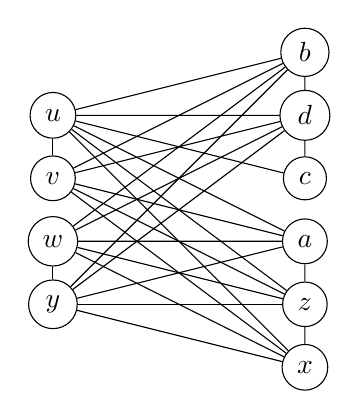
\begin{tikzpicture}[scale=0.8,every node/.style={circle,draw,minimum size=5mm}]
  \node (u) at (0, 4) {$u$};
  \node (v) at (0, 3) {$v$};
  \node (w) at (0, 2) {$w$};
  \node (y) at (0, 1) {$y$};

  \node (b) at (4, 5) {$b$};
  \node (d) at (4, 4) {$d$};
  \node (c) at (4, 3) {$c$};
  \node (a) at (4, 2) {$a$};
  \node (z) at (4, 1) {$z$};
  \node (x) at (4, 0) {$x$};

  \draw (u) -- (v);
  \draw (w) -- (y);
  \draw (b) -- (d);
  \draw (d) -- (c);
  \draw (a) -- (z);
  \draw (z) -- (x);
  \draw (u) -- (b);
  \draw (u) -- (d);
  \draw (u) -- (c);
  \draw (u) -- (a);
  \draw (u) -- (z);
  \draw (u) -- (x);
  \draw (v) -- (b);
  \draw (v) -- (d);
  \draw (v) -- (a);
  \draw (v) -- (z);
  \draw (v) -- (x);
  \draw (w) -- (b);
  \draw (w) -- (d);
  \draw (w) -- (a);
  \draw (w) -- (z);
  \draw (w) -- (x);
  \draw (y) -- (b);
  \draw (y) -- (d);
  \draw (y) -- (a);
  \draw (y) -- (z);
  \draw (y) -- (x);
\end{tikzpicture}
\quad
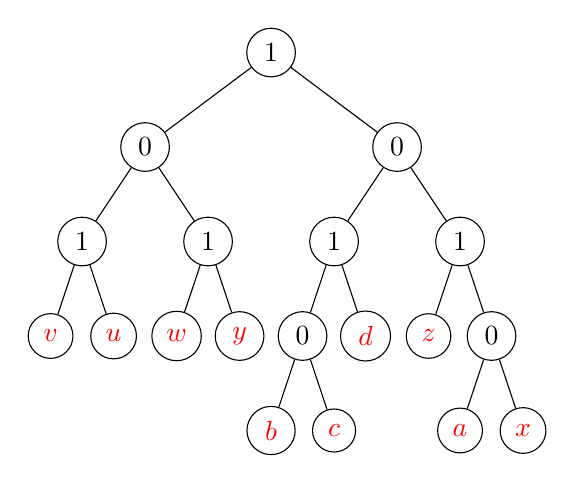
\begin{tikzpicture}[scale=0.8,every node/.style={circle,draw,minimum size=1mm},level distance=1.5cm,
  level 1/.style={sibling distance=4cm},
  level 2/.style={sibling distance=2cm},
  level 3/.style={sibling distance=1cm},
  level 4/.style={sibling distance=1cm}]
    
    \node {$1$}
        child { node {$0$}
            child { node {$1$}
                child { node {\textcolor{red}{$v$} }}
                child { node {\textcolor{red}{$u$}} }
            }
            child { node {$1$}
                child { node {\textcolor{red}{$w$} }}
                child { node {\textcolor{red}{$y$} }}
            }
        }
        child { node {$0$}
        child { node {$1$}
                child { node {$0$}
                    child { node {\textcolor{red}{$b$} }}
                    child { node {\textcolor{red}{$c$} }}
                }
                child { node {\textcolor{red}{$d$}}}
            }
        child { node {$1$}
        child { node {\textcolor{red}{$z$}}}
            child { node {$0$}
                child { node {\textcolor{red}{$a$} }}
                child { node {\textcolor{red}{$x$} }}
            }
        } 
        };
\end{tikzpicture}
    \caption{Cograph G and its cotree (taken from \cite{Bretscher2003ASL})}
    \label{fig:graph_example}
\end{figure} 